\section{Introduction}


\subsection{Body size trends in Neogene tortoises}

\begin{frame}{Terrestrial Tortoises}
\begin{picture}(300,250)
\put(0,75){
	\includegraphics<2>[height=5.5 cm]{pics/meiolania.png}
	\includegraphics<3->[height=5.5 cm]{pics/testudinidae.png}
}
\put(150,210){
%\fbox{
\begin{minipage}[t]{0.5\linewidth}
\begin{itemize}[<+->]
\p 2 clades:
\begin{itemize}
\p $\dagger$ Meiolaniidae (Australia, S-America)
\p[\pf] Lower Creataceous - Holocene
\p Testudinidae (extant terrestrial tortoises)
\p[\pf] oldest fossils from N-America + Europe (Eocene)
\end{itemize} 
%\p Meiolaniidae: extinct, used to be present in Australia + South America
%\p Testudinidae: comprise all extant terrestrial tortoises (America, Europe, Africa, Asia)
%\p Testudinidae: probably Asian origin, oldet fossils: North America + Europe
%\p today's most famous examples: giant tortoises (Galapagos + Aldabra) --> \textbf{map?}
\p throughout Earth's history: many large forms
\end{itemize}
\end{minipage}}
%}
\end{picture}
\end{frame}


\begin{frame}{Largest tortoises}
\begin{center}
	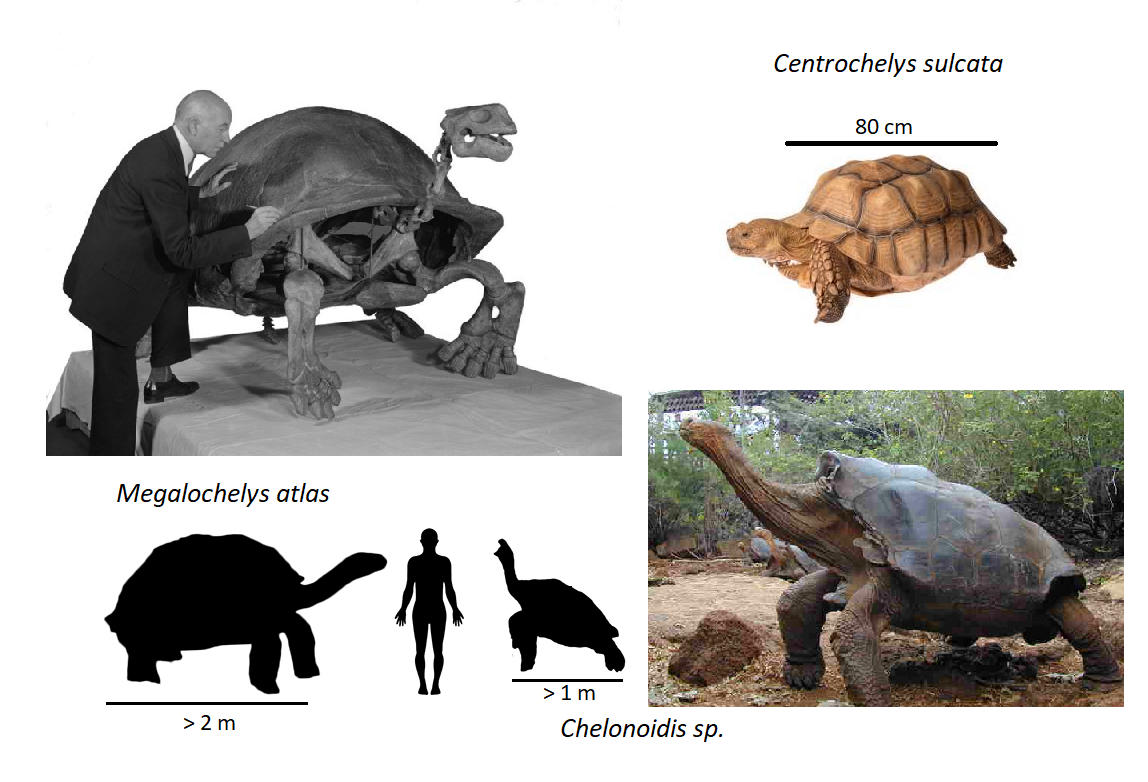
\includegraphics[width=\textwidth]{pics/gianttort.png}
\end{center}

\end{frame}

\begin{frame}{Megafauna}
\begin{picture}(300,250)
\put(0,100){
	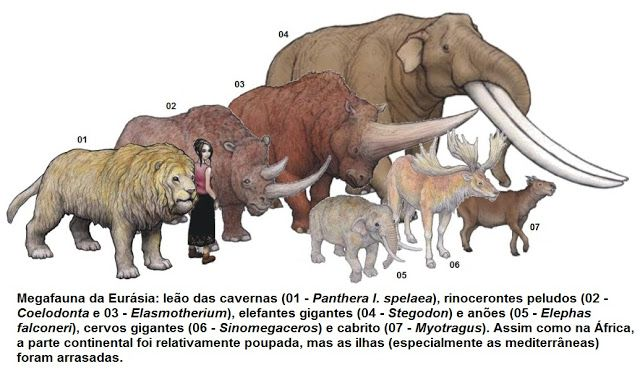
\includegraphics[width=5 cm]{pics/megafauna.png}
}
\put(150,210){
	%\fbox{
	\begin{minipage}[t]{0.5\linewidth}
	\begin{itemize}[<+->]
	\p animals with body mass $>$ 44 kg = megafauna
	\p mammalian megafauna: probably went extinct due to human influence!
	\p megafauna extinctions \pf humans or climate change?
	\end{itemize}
	\end{minipage}}
%}
\end{picture}
\end{frame}

%\begin{frame}{Pleistocene Extinctions}
%\begin{picture}(300,250)
%\put(0,90){
	%\missingfigure%\includegraphics[height=5 cm]{}
%}
%\put(150,210){
	%\fbox{
%	\begin{minipage}[t]{0.5\linewidth}
%	\begin{itemize}[<+->]
%	\p human influence
%	\p climate change
%	\p ...
%	\p ...
%	\end{itemize}
%	\end{minipage}}
%
%\end{picture}
%\end{frame}

%overview at the end of the introduction!
\begin{frame}
\begin{enumerate}[<+->]
\p Body size distribution of Testudinidae?
\bigskip
\p Body size differences on spatial/temporal scale?
\bigskip
\p General body size trends?
%--> or rather continuous gene flow or all 3 species arose from one shared ancestor?
%\bigskip
%\p Reasons for extinction?
%\bigskip
%\textcolor{gray}{....}
\end{enumerate}
\end{frame}
%}